\documentclass[letterpaper, 11pt, onecolumn, oneside]{article}

%%%%%%%%%%%%%%%%% Preamble %%%%%%%%%%%%%%%%%
% Packages
\usepackage[utf8]{inputenc}
\usepackage{textcomp}
\usepackage{graphicx}
\usepackage{amsmath}
\usepackage{amssymb}
\usepackage{fancyhdr}
\usepackage{xcolor}
\usepackage[margin=1in, headheight=26.2pt]{geometry}
\usepackage{mathptmx}
\usepackage[T1]{fontenc}
\usepackage[hidelinks]{hyperref}
\usepackage{pgfplots}
\usepackage{enumitem}
\usepackage{rotating}
\usepackage{pdfpages}
\usepackage{xspace}
\usepackage{caption}
\usepackage{subcaption}


% Variables
\newcommand{\assignmentname}{Project Report}
\newcommand{\assignmentdate}{December 12, 2019}

\DeclareMathOperator{\phase}{phase}
\DeclareMathOperator{\sinc}{sinc}
\DeclareMathOperator{\rect}{rect}
\DeclareMathOperator{\expectation}{E}
\DeclareMathOperator*{\argmin}{\arg\!\min}
\DeclareMathOperator*{\argmax}{\arg\!\max}

\newcommand{\expnumber}[2]{{#1}\mathrm{e}{#2}}
\newcommand{\MATLAB}{\mbox{\textsc{Matlab}}\xspace}
\newcommand{\norm}[1]{\left\lVert#1\right\rVert}
\newcommand{\expect}[1]{\expectation\left\{#1\right\}}

\graphicspath{{./figures/}{./code/}}

% Styling
\renewcommand{\familydefault}{\rmdefault}

\hypersetup{
    colorlinks=false,
    linkcolor=blue,
    urlcolor=blue,
}

\setlength{\parindent}{0pt}
\setlength{\parskip}{1em}

\definecolor{msu-maroon}{HTML}{660000}

\fancypagestyle{header}{
    \renewcommand{\headrulewidth}{2pt}
    \renewcommand{\headrule}{\hbox to\headwidth{\color{msu-maroon}\leaders\hrule height \headrulewidth\hfill}}
    \renewcommand{\footrulewidth}{2pt}
    \renewcommand{\footrule}{\hbox to\headwidth{\color{msu-maroon}\leaders\hrule height \footrulewidth\hfill}}
    \fancyhf{}
    \fancyhead[L]{\scriptsize CSE 6413}
    \fancyhead[C]{\Large {Computer Graphics}}
    \fancyhead[R]{\scriptsize Eric Farmer (EDF63)}
    \fancyfoot[L]{\scriptsize \assignmentname}
    \fancyfoot[C]{\scriptsize Page \thepage}
    \fancyfoot[R]{\scriptsize \assignmentdate}
}
\pagestyle{header}

% Info
\title{
    Ray Tracing\\
    \large{\assignmentname}
    }
\author{Eric Farmer \\ \href{mailto:edf63@msstate.edu}{\texttt{edf63@msstate.edu}}}
\date{\assignmentdate}


% Body
\begin{document}

% Make Title Page
\null  % Empty line
\nointerlineskip  % No skip for prev line
\vfill
\let\snewpage \newpage
\let\newpage \relax
\maketitle
\let \newpage \snewpage
\vfill
\clearpage

\section{Introduction}
Ray tracing is a rendering technique for generating images that simulates light propagating through space and shades objects based on complex inter-object interactions.
While computationally costly, ray tracing is capable of producing images with nearly-realistic quality.
Because of its ability to produce images with a very high degree of realism, it has become heavily integrated with the image and film industries.
Ray tracing is a powerful tool for integrating computer-generated graphics with real-life video captured on filming sets, which has allowed the film industry to continue producing higher quality films.
An example of the power of ray tracing is shown in Figure \ref{fig:nvidia-demo}, which is a computer-generated scene rendered using ray tracing with many advanced lighting components.

\begin{figure}[btp]
    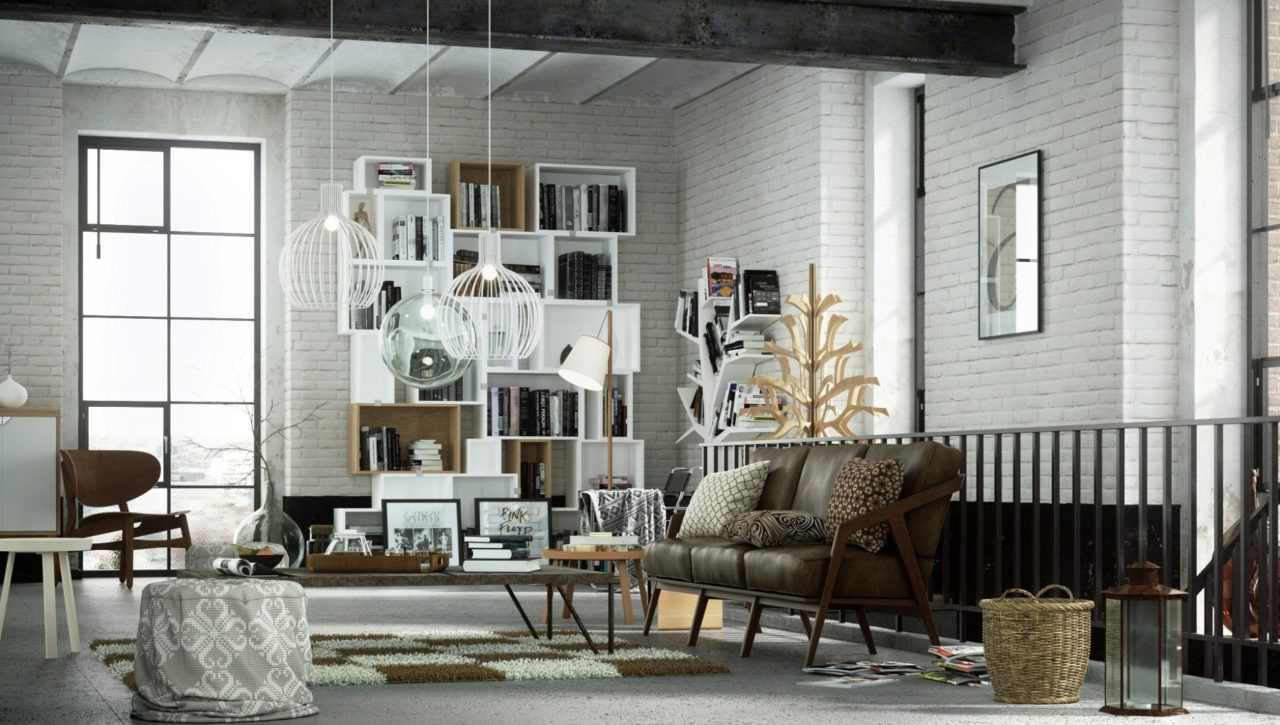
\includegraphics[width=0.8\textwidth]{nvidia-demo.jpg}
    \centering
    \caption{This computer-generated image shows the power of ray tracing \cite{caulfield2019}.}
    \label{fig:nvidia-demo}
\end{figure}

\section{Background}
One of the foundational tasks in computer graphics is rendering three-dimensional objects, which takes geometric objects arranged in three-dimensional space and produces a two-dimensional image that shows the objects as viewed from a certain viewpoint \cite{stevemarschner2015}.
This process takes as input a sete of 3-D objects and produces as output a 2-D array of pixels.
Rendering can occur in two orders -- object-order rendering and image-order rendering.
In object-order rendering, each object is processed and the pixels that it influences are calculated and updated.
In image-order rendering, each pixel is processed, and the objects that influence it are determined and the pixel value is found.
Ray tracing is an image-order rendering algorithm.

As an image-order rendering algorithm, the ray tracing algorithm begins by iterating over each pixel in the raster image.
For each pixel, the objective is to determine the geometric object observed by the ray emanating from the viewpoint in the direction of the pixel.
The object of interest is the object nearest the viewpoint because it occludes any objects farther into space along the ray's path.
After the object intersection is determined, the shading computation is performed.
The complexity of the shading model can vary, but an increase in complexity generally produces a higher quality rendering.

Thus, a ray tracer has three core components:
\begin{enumerate}
    \item ray generation, which computes the origin and direction of each pixel's viewing ray;
    \item ray-object intersection, which finds the closest object intersecting the viewing ray;
    \item shading, which computes the appropriate pixel color based on the results of the ray-object intersection \cite{stevemarschner2015}.
\end{enumerate}
These components are examined in more detail in Sections \ref{section:ray-generation}-\ref{section:ray-shading}.

One large drawback to ray tracing in its simplest form is the computation cost per raster image.
For a simple ray tracer, the performance depends on the number of rays being cast, which is influenced by the following:
\begin{enumerate}
    \item raster image resolution,
    \item multisample anti-aliasing level,
    \item number of objects and lights in the scene, and
    \item number of reflection bounces allowed.
\end{enumerate}
This performance quickly becomes undesirable for anything but the simplest scenes.
Techniques exist to improve this performance, but are not discussed in this document.

As demonstrated in Figure \ref{fig:nvidia-demo}, ray tracing is capable of generating incredibly realistic scenes.
This is done through complicated shading models that attempt to model the physical interactions of objects and light.

    \subsection{Ray Generation}
    \label{section:ray-generation}
        The concepts of ray tracing are rooted in the physical propagation of light rays throughout the environment.
        In reality, the light rays propagate from the light source throughout the scene until all the photonic energy has been absorbed.
        This method of propagating rays is called \textit{forward ray tracing}, and it has been implemented in computer graphics through Monte Carlo simulations.
        The advantage and disadvantage to this method is that the scene lighting is independent of the viewport.
        The light propagates throughout the scene until an equilibrium is reached.
        Thus, the advantage is that the camera can be positioned at any location and readily obtain the correctly lighted scene.
        The disadvantage is that it can take numerous iterations to reach a lighting equilibrium, and many light rays are unused because they never intersect the viewing plane.

        An alternative method, called \textit{backward ray tracing}, was developed to improve the rendering speed while maintaining the realistic lighting.
        In backward ray tracing, the theory is that only the light gathered at the camera is necessary, and it is unnecessary to light the entire scene to generate one raster image.
        Therefore, instead of shooting rays from each light source, the rays are shot from the camera through each pixel in the viewing plane.
        Because of its computational advantages, backward ray tracing has become the more common approach, and is usually the method referred to in the generic 'ray tracing' term.
        A comparison of the two methods of ray tracing is shown in Figure \ref{fig:forward-backward-tracing}.

        \begin{figure}
            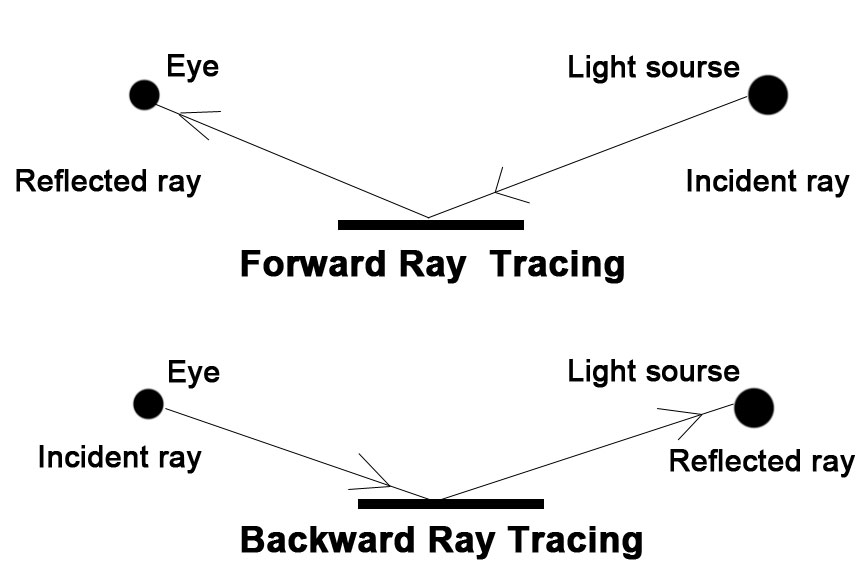
\includegraphics[width=0.4\textwidth]{forward-backward-tracing.jpg}
            \centering
            \caption{A comparison of forward and backward ray tracing methods. \cite{educba2019}.}
            \label{fig:forward-backward-tracing}
        \end{figure}

        During the Italian Renaissance, artists began designing using the principle of linear perspective to increase the realism of their work.
        The same principles are used today in computer graphics for the same reasons.
        Ray tracing can naturally incorporate one-point perspective projection by casting each ray from some camera point $\boldsymbol{e}$ through each pixel in the 2-D viewing plane.
        This process is seen in Figure \ref{fig:perspective-ray-generation}.

        Generating a ray requires two pieces of information -- the ray origin and the ray direction.
        To simplify the ray generation process, the scene is processed in camera space.
        This means that the camera is located at the origin $\boldsymbol{e}$ and is looking down the $-\boldsymbol{w}$ axis with the image plane aligned with the $\boldsymbol{uv}$ plane.
        The left and right image dimensions are defined by the edges of the image, $l$ and $r$, along the $\boldsymbol{u}$ axis.
        The top and bottom image dimensions are defined by the edges of the image, $t$ and $b$, along the $\boldsymbol{v}$ axis.
        Since the image plane is generally centered about $\boldsymbol{e}$, $l < 0 < r$ and $b < 0 < t$.
        The image must fit $n_x \times n_y$ pixels into the rectangle of size $(r-l) \times (t-b)$ with each pixel represented by its center.
        Therefore, the $(u,v)$ image plane coordinates of a pixel $(i,j)$ in the raster image are calculated by
        \begin{align} \label{eq:uv-calc}
            \begin{split}
                u &= l + \cfrac{(r-l)(i + 0.5)}{n_x} \\
                v &= b + \cfrac{(t-b)(j + 0.5)}{n_y}.
            \end{split}
        \end{align}
        Additionally, in perspective-based ray tracing, the image plane is offset from the camera location by some focal length $d$.
        With this information, the primary rays for the raster image can be generated using the following procedure:
        \begin{enumerate}
            \item Compute $u$ and $v$ from Equation (\ref{eq:uv-calc})
            \item The ray direction is $-d\boldsymbol{w} + u\boldsymbol{u} + v\boldsymbol{v}$ or, alternatively, $(-d,u,v)$ in camera space.
            \item The ray origin is $\boldsymbol{e}$.
        \end{enumerate}

        \begin{figure}
            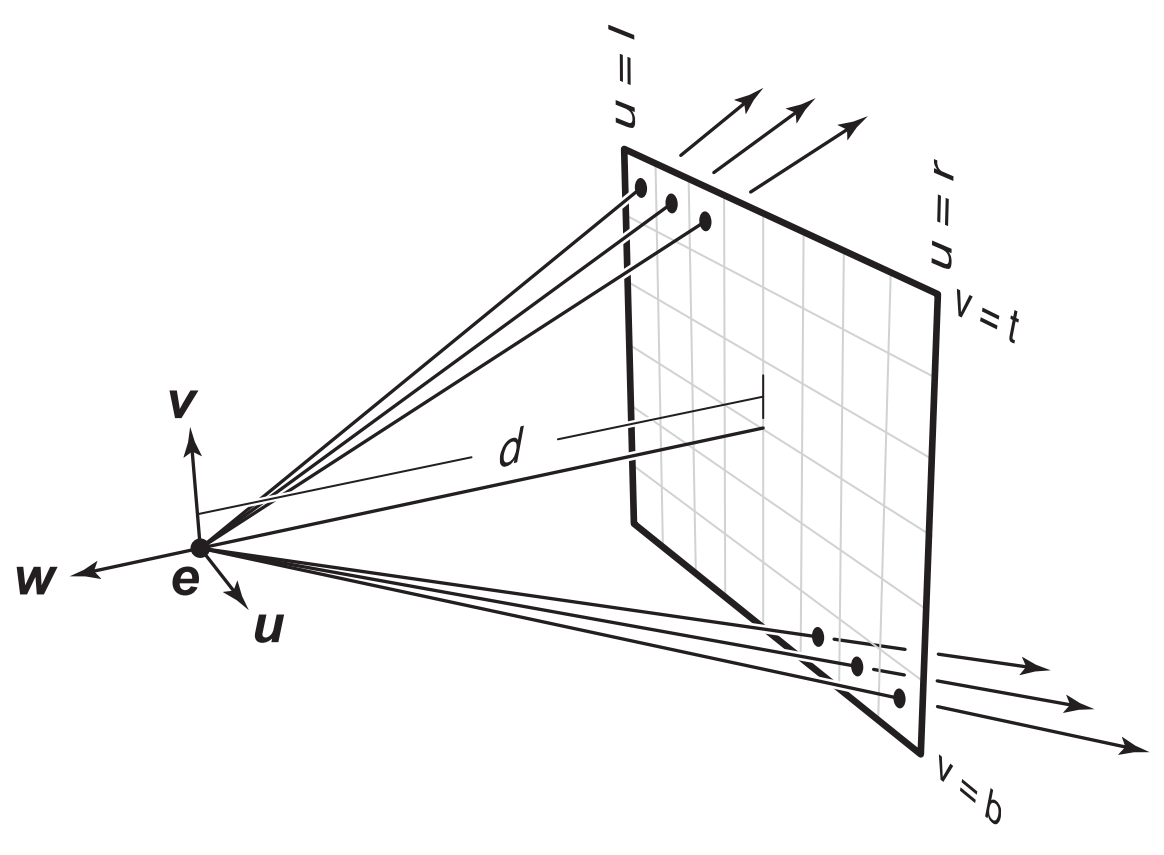
\includegraphics[width=0.6\textwidth]{perspective-ray-generation.png}
            \centering
            \caption{Primary ray generation for perspective projection. \cite{stevemarschner2015}}
            \label{fig:perspective-ray-generation}
        \end{figure}

    \subsection{Ray-Object Intersection}
    \label{section:ray-object-intersection}
        Once the primary viewing rays have been generated, the ray must be checked against the scene geometry to find the geometric object closest to the viewing plane.
        Many geometric objects allow for ray intersection calculations, but this project focused on triangle intersections.
        Recalling that the equation for a ray is
        \begin{align}
            \boldsymbol{p} = \boldsymbol{e} + t\boldsymbol{d},
        \end{align}
        where any point on the ray is calculated by adjusting $t$.
        Thus, the objective of ray-object intersection is to determine the value $t$, if it exists, for each geometric object.
        One method of calculating ray-triangle intersection is to utilize Barycentric coordinates.
        Thus, the intersection of a ray with a triangle is
        \begin{align} \label{eq:tri-intersection}
            \boldsymbol{e} + t\boldsymbol{d} = \boldsymbol{a} + \beta (\boldsymbol{b} - \boldsymbol{a}) + \gamma (\boldsymbol{c} - \boldsymbol{a}),
        \end{align}
        where $t$, $\beta$, and $\gamma$ are unknown values to calculate.
        In the Barycentric approach, the vertices of the triangle map out the plane that contains the triangle.
        Therefore, solving Equation (\ref{eq:tri-intersection}) can be broken down into two operations -- determining the offset $t$ where the ray intersects this plane and if that intersection point is inside the triangle.
        The intersection point is inside the triangle iff $\beta > 0$, $\gamma > 0$, and $\beta + \gamma < 1$.
        If no solutions exist, then the ray is parallel to the triangle plane or the triangle is degenerate.

        To solve Equation (\ref{eq:tri-intersection}) for the unknown variables, it can be rewritten as the system of linear equations
        \begin{align} \label{eq:linsys}
            \begin{bmatrix}
                x_a - x_b & x_a - x_c & x_d \\
                y_a - y_b & y_a - y_c & y_d \\
                z_a - z_b & z_a - z_c & z_d \\
            \end{bmatrix}
            \begin{bmatrix}
                \beta \\ \gamma \\ t
            \end{bmatrix}
            =
            \begin{bmatrix}
                x_a - x_e \\
                y_a - y_e \\
                z_a - z_e
            \end{bmatrix}.
        \end{align}
        The variables can be solved for using Cramer's rule.
        Substituting for the standard column-order dummy variables and solving gives
        \begin{align}
            \beta &= \cfrac{j(ei -hf) + k(gf-di) + l(dh-eg)}{M} \\
            \gamma &= \cfrac{i(ak-jb) + h(jc-al) + g(bl-kc)}{M} \\
            t &= -\cfrac{f(ak-jb) + e(jc-al) + d(bl-kc)}{M},
        \end{align}
        where
        \begin{align}
            M = a(ei-hf) + b(gf-di) + c(dh-eg).
        \end{align}

        The speed of this algorithm can be improved by using early termination.
        Since the ray offset $t$ must fall within some bounds, $t$ may be computed first to determine if the intersection occurs at a point closer to the ray origin than already seen.
        If not, then $\beta$ and $\gamma$ are not calculated.
        Additionally, early termination may be performed on $\gamma$ to ensure $\gamma \in (0,1)$.

        Using the Barycentric coordinates where $\alpha = 1-\beta-\gamma$, interpolation can be performed at the intersection point.
        This interpolation allows the intersection point to return its interpolated position, normal vector, and colors.
        These values are useful in the next stage of ray tracing -- shading.

    \subsection{Shading Model}
    \label{section:ray-shading}
        The Blinn-Phong shading model is used to determine the color at each pixel of a raster image.
        For ray tracing, the total light intensity $I$ received at the surface is
        \begin{align}
            I = I_a + I_d + I_s + I_e + I_r + I_t,
        \end{align}
        where
        \begin{align}
            I_a &= k_a\left(I_{a_{global}} + \sum_i I_{a_i}\right) \\
            I_d &= \sum_i \cfrac{k_d}{a + bD_i + cD_i^2} \left(\boldsymbol{l}_i \cdot \boldsymbol{n}\right) I_{d_i}\\
            I_s &= \sum_i \cfrac{k_s}{a + bD_i + cD_i^2} \left(\boldsymbol{n} \cdot \boldsymbol{h_i}\right)^s I_{s_i}\\
            I_e &= k_e \\
            I_r &= \cfrac{k_r}{a + bD_r + cD_r^2} I\left(\boldsymbol{u}_r\right) \\
            I_t &= \cfrac{k_t}{a + bD_t + cD_t^2} I\left(\boldsymbol{u}_t\right).
        \end{align}
        The vectors are shown in Figure \ref{fig:blinnphong-vectors}, and
        \begin{align}
            \boldsymbol{h} &= \cfrac{\boldsymbol{l}_i + \boldsymbol{v}}{\norm{\norm{\boldsymbol{l}_i + \boldsymbol{v}}}} \\
            \boldsymbol{u}_r &= \boldsymbol{u} - \left(2\boldsymbol{u} \cdot \boldsymbol{n}\right) \boldsymbol{n} \\
            \boldsymbol{u}_t &= \cfrac{\eta_i}{\eta_t}\boldsymbol{u} - \left(\cos{\theta_t} - \cfrac{\eta_i}{\eta_t}\cos{\theta_i}\right) \boldsymbol{n}.
        \end{align}
        An advanced version of this shading model is shown in Figure \ref{fig:adv-shading-model-vectors}, but not used in this project.

        \begin{figure}[ht]
            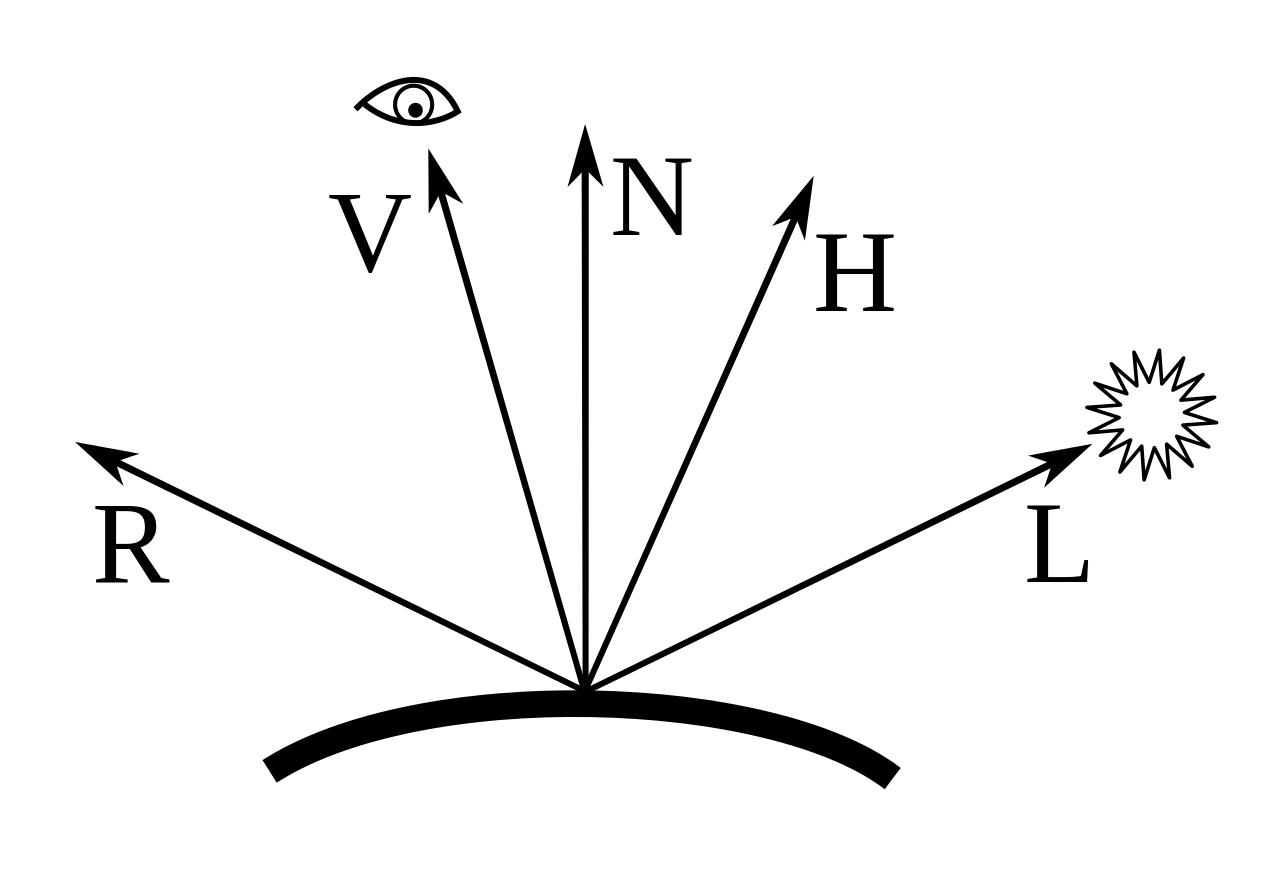
\includegraphics[width=0.4\textwidth]{blinnphong-vectors.png}
            \centering
            \caption{The vectors associated with the Blinn-Phong shading model \cite{kraus2011}.}
            \label{fig:blinnphong-vectors}
        \end{figure}

        \begin{figure}[ht]
            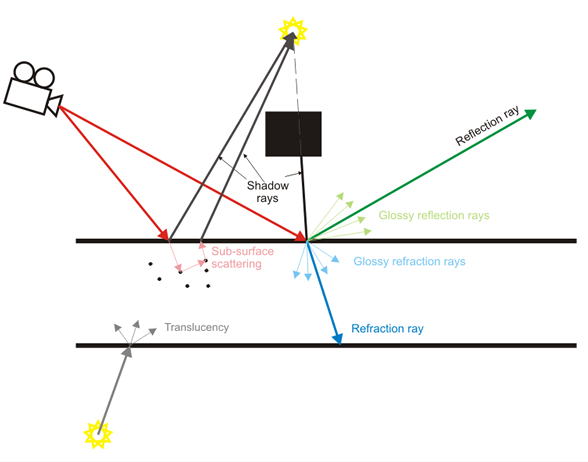
\includegraphics[width=0.65\textwidth]{ray-tracing-shading-model.png}
            \centering
            \caption{Shading vectors associated with advanced shading models \cite{chaosShading}.}
            \label{fig:adv-shading-model-vectors}
        \end{figure}


\section{Results}
    The original goal for this project was to render the MINI Cooper model used during class in the Cornell box.
    However, due to the amount of rendering time required, the MINI Cooper model has not completed rendering in time for this report.
    In it's place, a reflective box was placed in the Cornell box.

    The first step in the process was generating the Cornell box with simple ambient lighting.
    Numerous difficulties arose here due to generating the box geometry by hand.
    First, the bottom and top planes of the box were accidently placed at different heights than the walls, which led to an awkward gap.
    After fixing this, a ray-traced Cornell box with ambient lighting was generated, shown in Figure \ref{fig:box-ambient}.
    To improve the render quality, 16x multisample antialiasing was added and used for all the images shown in this report.

    The next step was to add diffuse lighting to the raytracer.
    Diffuse lighting requires a light source.
    For simplicity, the first light source implemented was a directional light source.
    The light source for the following renderings was oriented toward $[-1, -1, -1]$.
    While attempting to add diffuse lighting, it was discovered that the hand-generated point normals for the Cornell box model were incorrect.
    This led to incorrect diffuse lighting, and difficulty in debugging.
    However, after this problem was remedied, the Cornell box was rendered again with ambient and diffuse lighting from a directional light, shown in Figure \ref{fig:box-ambient-diffuse}.

    To complete the standard Phong lighting model, specular lighting was added.
    One difficulty encountered here was that the pixel colors were now exceeding one, which was causing a wrap around to occur when converting from float64 to uint8.
    This caused the specular areas to appear black instead of white.
    This was remedied by clamping all values over 1.0 to 1.0.
    The result is shown in Figure \ref{fig:box-phong}.

    \begin{figure}
    \centering
    \begin{subfigure}{.3\textwidth}
      \centering
      
\includegraphics[width=.85\linewidth]{box-16xAA-ambient.png}
      \caption{Ambient}
      \label{fig:box-ambient}
    \end{subfigure}%
    \begin{subfigure}{.3\textwidth}
      \centering
      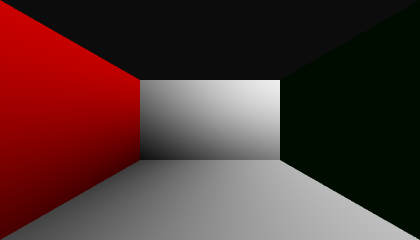
\includegraphics[width=.85\linewidth]{box-16xAA-directional-ambient-diffuse.png}
      \caption{Ambient \& Diffuse for Directional Light}
      \label{fig:box-ambient-diffuse}
    \end{subfigure}%
    \begin{subfigure}{.3\textwidth}
      \centering
      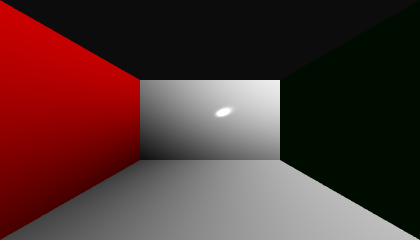
\includegraphics[width=.85\linewidth]{box-16xAA-directional-phong.png}
      \caption{Phong Lighting for Directional Light}
      \label{fig:box-phong}
    \end{subfigure}
    \caption{The development of the ray tracing algorithm with the Cornell box.}
    \end{figure}

    With Phong light stably implemented, the next step was to use the power of ray tracing to generate shadows.
    The result of adding shadows with a directional light is shown in Figure \ref{fig:box-shadows}.
    Due to the sharp edges in the scene and simple method used for calculating shadows, the shadows look unrealistic.
    A better approach would have been to use soft shadows by multisampling the shadow feeler ray.

    The next task was to generate reflections.
    This required an extension to the geometry framework to incorporate the reflective properties of the materials.
    For the Cornell box, the bottom and back faces were set as reflective.
    The integration of reflections went fairly smoothly, and the results of adding reflective lighting to the Cornell box is shown in Figure \ref{fig:box-reflective}

    \begin{figure}
    \centering
    \begin{subfigure}{.5\textwidth}
      \centering
      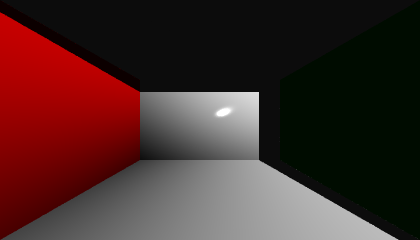
\includegraphics[width=.85\linewidth]{box-16xAA-directional-phong-shadows.png}
      \caption{Ambient}
      \label{fig:box-shadows}
    \end{subfigure}%
    \begin{subfigure}{.5\textwidth}
      \centering
      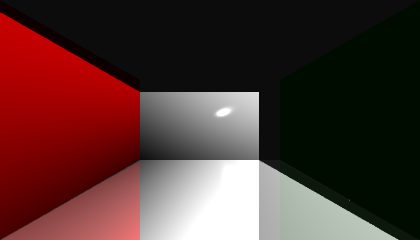
\includegraphics[width=.85\linewidth]{box-16xAA-directional-phong-shadows-reflections.png}
      \caption{Shadows \& Reflections for Directional Light}
      \label{fig:box-reflective}
    \end{subfigure}
    \caption{The addition of more complex lighting.}
    \end{figure}

    With the demonstration of a successful lighting model, the raytracer was expanded to process multiple lights.
    The addition of multiple lights was simple because it had been designed for from the start.
    The only change made was that more lights were added to the scene when it was loaded.
    The light sources for Figure \ref{fig:twolights} were $[-1,-1,-1]$ and $[1, 1, -1]$.
    The light sources for Figure \ref{fig:threelights} extended the two ligth case by adding a light towards $[0, 1, -1]$.

    \begin{figure}
    \centering
    \begin{subfigure}{.5\textwidth}
      \centering
      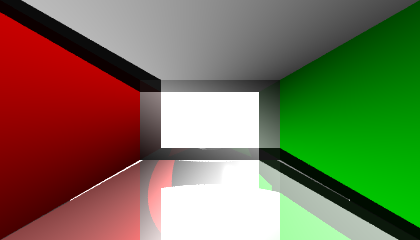
\includegraphics[width=.85\linewidth]{box-16xAA-2xML-phong-shadows-reflections.png}
      \caption{Two Directional Lights}
      \label{fig:twolights}
    \end{subfigure}%
    \begin{subfigure}{.5\textwidth}
      \centering
      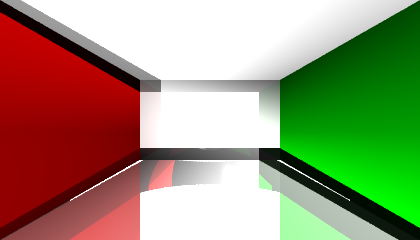
\includegraphics[width=.85\linewidth]{box-16xAA-3xML-phong-shadows-reflections.png}
      \caption{Three Directional Lights}
      \label{fig:threelights}
    \end{subfigure}
    \label{fig:multilights}
    \caption{The addition of more complex lighting.}
    \end{figure}

    Finally, to increase the complexity of the scene, a reflective box was added inside the Cornell box.
    This process was merely tedious to generate another set of geometry for the box.
    The result was impressive though, and can be seen in Figure \ref{fig:multibox}.

    \begin{figure}[ht]
        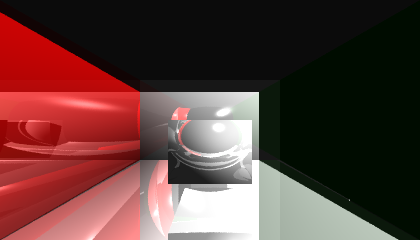
\includegraphics[width=0.65\textwidth]{box-16xAA-1xML-multibox-full.png}
        \centering
        \caption{Reflective multibox rendering with 16xMSAA and a single directional light source.}
        \label{fig:multibox}
    \end{figure}


\section{Conclusion and Future Work}
    In conclusion, this project successfully demonstrated some of the fundamental features of ray tracing for producing 2-D raster images from 3-D scenes.
    While the final results used a simpler model than desired, it still demonstrated the lighting effects intended.


    The future work for this project can be split into three categories -- optimization, usability, and realism.
    Work in the optimization category attempts to improve the performance of the program in speed or memory.
    The usability category attempts to improve the compatibility of the program with various model formats.
    Improvements to realism attempt to render the scene using more advanced techniques to generate higher quality images.
    The following list shows a breakdown of the future work for this project:
    \subsection{Optimization Improvements}
        \paragraph{Bounding Box Intersections}
        This improvement checks each mesh object by its bounding box before iterating over the contained geometry.
        Using this approach, more complex scenes can be rendered faster because each geometric object is not checked for each ray.

        \paragraph{Multiprocessing}
        This improvement is to parallelize the primary ray casting.
        Each primary ray is independent of all other primary rays, so multiple pixels may be calculated in parallel.
        The simplest implementation here is to utilize the central processing unit cores available.
        More advanced implementations could leverage graphics processing units to achieve much higher parallelization at the cost of redesigning to account for the memory management necessary.

        \paragraph{Spatial Search Structures}
        Using a data structure that supports spatial search can improve the search time for geometric objects during the intersection test.
        One commonly used structure is Kd-trees.

    \subsection{Usability Improvements}
        \paragraph{Additional Geometries}
        Currently, the program lacks the ability to process anything except triangles.
        The addition of various geometric primitives would increase the usability of the program.
        Using the appropriate geometric representation of objects can also increase render speed.
        For example, a circle composed of triangle is a lot of objects to check for intersection, whereas a circle object would be only one intersection check.

        \paragraph{Extended File Formats}
        The program lacks the ability to load models from standard file formats.
        This improvement would allow the ray tracer to interact with current modeling software more easily, which allows for more complex scene generation.

    \subsection{Realism Improvements}
        The ray tracer can be expanded to do soft shadows and more advanced lighting models.
        Additionally, higher fidelity models are required to calculate some lighting effects.

\clearpage
\bibliography{edf63_ProjectReport}
\bibliographystyle{ieeetr}
\nocite{*}

\clearpage
\vspace*{\fill}
\section*{\centering Assignment Code}

\begin{center}
The source code for this assignment is hosted on GitHub.

\texttt{https://github.com/WhoFama24/cse6413-raytracer.git}
\end{center}
\vspace*{\fill}

\end{document}
